%%%%%%%%%%%%%%%%%%%%%%%%%%%%%%%%%%%%%%%%%%%%%%%%%%%%%%%%%%%%%%%%%%%%%%%%%%%%%%%%%
%% Paper B -- Target: Environment Systems and Decisions (Springer), Q2
%% Carbon-aware storage-architecture selection for image-based time-series in
%% green IoT (three-way: MongoDB vs PostgreSQL-BYTEA vs PostgreSQL+MinIO).
%%
%% This manuscript consolidates two conference drafts (Postgre-vs-MongoDB and
%% Postgre-vs-Postgre+MinIO) into ONE three-way study and is now backed by a unified,
%% object-oriented benchmark harness that measures per-resolution carbon
%% DIRECTLY (one CodeCarbon tracker per engine x dimension x resolution) over a
%% single 360p->6K sweep with a common retrieval workload across all engines.
%% Data: ../data/ (collage, i9), ../data_collage_i7/, ../data_frames_*/ (real case)
%% Figures: ../figures/   Harness: ../code/   Recorder: ../code_realcase/
%%%%%%%%%%%%%%%%%%%%%%%%%%%%%%%%%%%%%%%%%%%%%%%%%%%%%%%%%%%%%%%%%%%%%%%%%%%%%%%%%

\documentclass[pdflatex,sn-basic]{sn-jnl}% Basic Springer Nature reference style (name-year). Add ",Numbered" if ESD requires numbered citations.

\usepackage{graphicx}%
\usepackage{multirow}%
\usepackage{amsmath,amssymb,amsfonts}%
\usepackage{booktabs}%
\usepackage{xcolor}
\usepackage{array}
\newcolumntype{L}[1]{>{\raggedright\arraybackslash}p{#1}}%
\usepackage{textcomp}%
\usepackage{manyfoot}% required by sn-jnl (table footnotes / \SetFootnoteHook)
\usepackage{listings}%

\graphicspath{{figures/}{../figures/}}

% A small MongoDB-shell (JavaScript) language, since the listings package
% ships SQL but not JavaScript; visual styling is set in \lstset below.
\lstdefinelanguage{MongoJS}{
  morekeywords={db, var, let, const, function, return, true, false, null, new,
    ISODate, BinData, createCollection, createIndex, insertMany, find, sort,
    limit, aggregate, timeseries, timeField, metaField, granularity},
  sensitive=true,
  morecomment=[l]{//},
  morecomment=[s]{/*}{*/},
  morestring=[b]"
}

\lstdefinelanguage{PgSQL}[]{SQL}{
  morekeywords={BIGSERIAL,TIMESTAMPTZ,BYTEA,BIGINT,INTEGER,TEXT},
  morecomment=[l]{--}
}

\lstset{
  basicstyle=\ttfamily\scriptsize,
  keywordstyle=\color{blue}\bfseries,
  commentstyle=\color{gray}\itshape,
  stringstyle=\color{red},
  showstringspaces=false,
  breaklines=true,
  frame=lines,
  numbers=left,
  numberstyle=\tiny\color{gray},
  numbersep=6pt,
  xleftmargin=1.4em,
  framexleftmargin=1.4em,
  backgroundcolor=\color{lightgray!10},
  tabsize=2,
  columns=fullflexible}

% Float placement: with many floats the defaults push them to the
% end of the document. These values let LaTeX place them near their text.
\setcounter{topnumber}{3}
\setcounter{bottomnumber}{2}
\setcounter{totalnumber}{4}
\renewcommand{\topfraction}{0.9}
\renewcommand{\bottomfraction}{0.8}
\renewcommand{\textfraction}{0.07}
\renewcommand{\floatpagefraction}{0.75}

\raggedbottom

\begin{document}

\title[Carbon-aware storage selection for image-based time-series in green IoT]{Carbon Footprint and Carbon-Aware Selection of Document-Oriented, Relational, and Hybrid Object-Relational Storage for Image-Based Time-Series Workloads in Green IoT}

% Author, affiliation, and email details removed for double-anonymous review.
% The starred forms mark a corresponding author, which makes the class emit a
% "Corresponding author(s). E-mail(s):" line. Even with an empty \email{} that
% line survives into the PDF, and the submission system's automated check reads
% it as an email field. Unstarred, with no \email at all, it disappears.
\author[1]{\sur{[Hidden for Double-blind Review]}}

\affil[1]{\orgname{[Hidden for Double-blind Review]}}

\abstract{Building-monitoring systems increasingly keep image streams with timestamped metadata in an always-on data tier, which makes the storage backend a sustainability decision. We measured the carbon footprint of three storage architectures for image-based time-series workloads: the document database MongoDB, with images inside each record; PostgreSQL with TimescaleDB, with images in a binary column; and a hybrid that keeps metadata in PostgreSQL and images in the MinIO object store. A separate energy tracker covered every architecture, operation, and resolution from 360p to 6K. The results show a payload-dependent crossover with no universal winner. Counting insertion, bulk retrieval, and latest-frame reads equally, MongoDB is greenest for small payloads and the hybrid from 4K, roughly halving the carbon of inline storage. Under its default time-series bucketing MongoDB cannot store 6K frames at all, and on a memory-constrained host it failed from 4K. Real camera frames are several times smaller than the test images at the same resolution, so the derived decision rule is keyed to measured payload, operation profile, and retention, with a procedure for locating its boundaries elsewhere. A sensitivity analysis shows that grid intensity and facility overhead cannot change the ranking, that host, image corpus, and operation mix move the crossover rather than the ordering, and that the embodied carbon of retained frames can outweigh write energy and reverse close choices. The measurements cover only the storage tier, one host at a time with one client; memory power is estimated; and the annual figures are projections rather than measured savings.}

\keywords{carbon footprint, green computing, sustainable IoT, time-series databases, image-based storage, decision support, life-cycle assessment, software carbon intensity, PostgreSQL, MongoDB, MinIO}

\maketitle

%%=====================================================================%%
\section{Introduction}\label{sec:introduction}
%%=====================================================================%%

Smart-building and facility-monitoring systems increasingly combine conventional telemetry with image streams from embedded cameras, smart doorbells, inspection devices, and other Internet-of-Things (IoT) edge devices~\citep{bajera_iot_smart_buildings,alfuqaha_iot_survey}. These applications retain the images together with timestamps, device identifiers, and other metadata, so that operators can inspect the latest frame, replay recent events, or query activity over time~\citep{ceec_tsdb_review,jensen_tsms_survey}. Because the \emph{data tier} that stores and serves this information runs continuously, its electricity use contributes directly to the operational carbon footprint of the building or infrastructure~\citep{nerc_tsdb_survey}. Data centres and on-premises information-technology (IT) equipment already account for a significant and growing share of electricity demand~\citep{masanet_datacenter_energy,shehabi_us_datacenter}, and as green-building standards begin to count the carbon cost of IT, the choice of storage system becomes an environmental and infrastructure-management decision as well as a technical one~\citep{ieee_ce_definition}.

Organisations typically reuse general-purpose databases for this role~\citep{intuz_iot_databases}, and three architectures dominate practice, differing chiefly in where the image goes. \emph{MongoDB}~\citep{mongodb_official}, a document database with native Time-Series Collections, keeps it inside the document in its BSON encoding~\citep{mongodb_bson_spec}, written by the WiredTiger engine~\citep{mongodb_wiredtiger_storage} after Snappy compression~\citep{google_snappy}. \emph{PostgreSQL}~\citep{postgresql_official}, with the TimescaleDB extension~\citep{timescaledb_official} for time-based partitioning, holds it in a column that TOAST (The Oversized-Attribute Storage Technique) moves out of line when it is large~\citep{postgresql_toast_docs}. A widely used \emph{hybrid} keeps only the metadata in PostgreSQL and the image in an object store such as MinIO~\citep{minio_official} or Amazon S3~\citep{aws_s3_official}. Because these designs move, copy, and compress the image differently, their energy use can diverge as payload size grows.

Existing time-series benchmarks target lightweight numeric events~\citep{tsbs,cratedb_ts_benchmark,diva_timescaledb_mongodb_eval}; they rarely evaluate multi-megabyte image payloads, and even more rarely report energy use or carbon-dioxide-equivalent (CO\textsubscript{2}eq) emissions. Image-heavy IoT deployments are therefore left without evidence on which storage architecture minimises carbon, and under which operating conditions, although a storage system's behaviour changes with payload size, so a conclusion drawn at one resolution need not hold at another.

This paper addresses the following research question: \emph{What is the carbon footprint of document-oriented, relational, and hybrid object-relational storage for image-based time-series workloads across increasing camera resolutions, and how should an operator choose among them to minimise emissions in green IoT infrastructure?} We answer it through three sub-questions:
\begin{itemize}
  \item[RQ1] How do the operational carbon footprints of the three architectures compare across payload sizes and operations? (Sections~\ref{subsec:insert}--\ref{subsec:carbon} and~\ref{subsec:bson})
  \item[RQ2] How far do the ordering and its limits hold across hosts, payload corpora, and the assumptions of the analysis? (Sections~\ref{subsec:grid}, \ref{subsec:twohosts}--\ref{subsec:sizevsres} and Online Resource~2)
  \item[RQ3] How should an operator choose an architecture to lower emissions, and what does the saving mean for carbon accounting and policy? (Sections~\ref{sec:framework} and~\ref{subsec:accounting})
\end{itemize}
To answer them, we benchmark the three architectures at eight resolutions from 360p to 6K with JPEG images~\citep{wallace_jpeg}, each in its own Docker container~\citep{docker_official}, and measure energy with CodeCarbon~\citep{codecarbon}, which reads the processor's Running Average Power Limit (RAPL) counters~\citep{david_rapl} and estimates memory power. Unlike earlier conference studies [hidden for double-blind review], every resolution has its own energy tracker and all three systems share one read workload. We frame storage selection as an \emph{environmental-systems decision} that weighs operational and embodied carbon against performance and operational complexity for a deployment's payloads and electricity grid. The contributions are:

\begin{itemize}
  \item A three-way, directly measured carbon-footprint comparison of MongoDB, PostgreSQL-BYTEA (PostgreSQL storing each image inline in a \texttt{BYTEA} column), and PostgreSQL+MinIO under identical image-based time-series workloads from 360p to 6K.
  \item Evidence of a \emph{payload-dependent emission crossover}, with MongoDB greenest at standard resolutions and the hybrid at high ones, and two infeasibility results: under the default bucketing of a native time-series collection MongoDB cannot store 6K frames at all, because the bucket breaches the 16~mebibyte (MiB) limit on a BSON document, and on a memory-constrained host it fails from 4K.
  \item An environmental analysis beyond a performance benchmark: Software Carbon Intensity (SCI), the Green Software Foundation's rate of carbon per unit of useful work~\citep{gsf_sci}, whose version~1.0 is ISO/IEC~21031:2024~\citep{iso_iec_21031_sci}; a sensitivity analysis of the ranking to the operation mix, measurement variability, grid intensity~\citep{owid_carbon_intensity}, facility overhead, and the embodied carbon of retained storage~\citep{tannu_ssd_embodied,gupta_chasing_carbon}; an annual projection for a real deployment; and an interpretation of the savings for carbon accounting, markets, and policy (Section~\ref{subsec:accounting}).
  \item A \emph{carbon-aware decision framework} that maps measured payload size and workload emphasis to the lowest-emission architecture, with a short calibration procedure for locating its boundaries at another site.
\end{itemize}

To our knowledge, no earlier study measured the carbon of individual storage operations for multi-megabyte payloads, reported either infeasibility result, or keyed a storage-selection rule to measured payload with a procedure for applying it elsewhere. The results also travel. They are expressed per frame and per 1{,}000 frames (SCI), so they rescale to any grid; the ranking is the same under seven national grids from 41 to 713~g~CO\textsubscript{2}eq/kWh (Section~\ref{subsec:grid}); and the calibration procedure is the same at any site, which measures its own payload and locates its own boundaries.

%%=====================================================================%%
\section{Related Work}\label{sec:related_work}
%%=====================================================================%%

\subsection{Time-series storage}
Time-series databases serve data that mostly arrives in timestamped order and is rarely modified, sustaining append-oriented ingestion through time-based partitioning, compression, and layouts that reduce write amplification~\citep{dewaal_timeseries_survey,jensen_tsms_survey}. TimescaleDB~\citep{timescaledb_official} adds time-based partitioning to PostgreSQL, and MongoDB~\citep{mongodb_official} offers native Time-Series Collections that bucket many measurements into compacted documents~\citep{mongodb_timeseries_collections_guide,mongodb_ts_best_practices}.

\subsection{Benchmarks and the binary-payload gap}
Most comparative benchmarks target lightweight scalar data: TSBS~\citep{tsbs} uses small DevOps and telemetry records, CrateDB's benchmark~\citep{cratedb_ts_benchmark} numeric IoT metrics, and \citet{diva_timescaledb_mongodb_eval} numerical sensor workloads. None of the benchmarks reviewed here characterises multi-megabyte image payloads or reports energy or emissions (Table~\ref{tab:relwork}); we make no claim beyond the studies in that table. For large values, PostgreSQL's TOAST~\citep{postgresql_toast_docs} moves them out of line but keeps them within the database's transactional machinery; MongoDB stores binaries inline in BSON documents~\citep{mongodb_bson_spec}, since its large-file alternative, GridFS~\citep{mongodb_gridfs}, is incompatible with Time-Series Collections~\citep{mongodb_ts_limitations}; and object stores such as MinIO~\citep{minio_official} stream large objects while a relational system keeps only the metadata. The trade-off is one transactional path for everything against separating metadata management from binary transport. Where large objects belong is an older question: comparing SQL Server with the NTFS filesystem by throughput, \citet{sears_blob_filesystem} found objects under 256~KB better kept in the database and over 1~MB in the filesystem, with write intensity and the age of the store deciding in between. That is the nearest precedent for our crossover, though it measured no energy.

\subsection{Carbon footprint of computing}
Green Algorithms~\citep{lannelongue_green_algorithms} and work on the energy cost of large-scale computation~\citep{strubell_energy_nlp} established footprint estimation for computing, and CodeCarbon~\citep{codecarbon} implements it from machine-level measurements and grid intensity. Beyond operational carbon, a growing literature treats \emph{embodied} carbon, the emissions of manufacturing hardware, as a first-class concern~\citep{gupta_chasing_carbon}, with flash storage a notable contributor~\citep{tannu_ssd_embodied}. Facility accounting multiplies computing energy by the Power Usage Effectiveness (PUE), the ratio of a data centre's total energy to that reaching its IT equipment~\citep{shehabi_us_datacenter,masanet_datacenter_energy}, and the Software Carbon Intensity specification~\citep{gsf_sci} standardises reporting per unit of useful work. Within database systems, \citet{harizopoulos_energy_dbms} argue that data-management software, not hardware alone, will decide energy efficiency, and that the most efficient operating point is not the best-performing one; measuring a database server, \citet{tsirogiannis_db_server_energy} found the opposite within a single node. Our results side with the latter for the long operations that dominate a monitoring workload, but not for the shortest reads (Section~\ref{subsec:winners}). Little of this work applies per-operation carbon accounting to binary time-series storage.

\subsection{Environmental decision analysis in this journal}\label{subsec:esd}
The framework proposed here is a decision-analysis instrument, and it follows a line of work in this journal that couples measured evidence to a selection rule. \citet{bajwa_material_selection_mcdm} survey multi-criteria decision making for material selection in construction and identify a recurring weakness: criteria are often drawn from the literature rather than measured in the deciding organisation's own context, which limits transferability. We respond by making the decision variable, payload size, directly measurable by the adopter. \citet{kraft_lca_railway_sensitivity} shows, in a life-cycle assessment of lightweight railway vehicles, that sensitivity analysis is what separates a robust design conclusion from an artefact of assumed parameters; the sensitivity analysis of Section~\ref{subsec:grid} plays that role here.

Closer to our deployment, \citet{adams_smart_home_energy} estimate a smart home's energy consumption by data-driven simulation, treating the building's instrumentation as the object of analysis; the tier that stores what the instrumentation records lies outside their models, and a storage decision alone can roughly halve its carbon. \citet{singh_iot_self_healing} and \citet{radanliev_iot_edge_risk} address the operational integrity of IoT systems, through self-healing log analytics and real-time risk at the edge, and both presuppose a data tier that durably retains device output; we supply the environmental cost of that presupposition. Finally, \citet{alessa_demand_response_review} review price-driven energy management and demand response, which shift load in time to exploit a varying grid. Because emissions are energy multiplied by grid intensity, such shifting rescales every architecture equally and cannot change which one to choose (Section~\ref{subsec:grid}); the saving must come from the architecture itself.

\subsection{Gaps addressed}
Three gaps follow from this review, one for each research question. Time-series benchmarks use small scalar rows and report no energy, and the classic study of where large objects belong measured throughput alone, so nothing establishes how the carbon of storing multi-megabyte payloads compares across architectures (RQ1). We found no study that tests how far such a ranking survives a change of host, of payload realism, or of the assumptions behind the carbon figures (RQ2). And carbon-accounting methods work above the level of a storage operation, so they cannot tell an operator which architecture to pick, while no published procedure for choosing a store carries over from one site to another (RQ3).

\begin{table}[htbp]
\caption{Representative time-series benchmarks versus this work, with what each concludes and what changes once payloads are large enough for the engine's internal layout to dominate.}\label{tab:relwork}
\footnotesize
\setlength{\tabcolsep}{3pt}
\begin{tabular}{@{}L{0.155\textwidth}L{0.115\textwidth}L{0.065\textwidth}L{0.115\textwidth}L{0.075\textwidth}L{0.315\textwidth}@{}}
\toprule
Study & Payload type & Max payload & Engines & Energy / CO\textsubscript{2}? & What it concludes / what this work changes \\
\midrule
TSBS~\citep{tsbs} & numeric/scalar & $\sim$KB & multiple TSDBs & No & Ranks engines on small scalar rows, where per-row overhead dominates; the ranking inverts once the payload governs the write path. \\
CrateDB~\citep{cratedb_ts_benchmark} & numeric IoT metrics & $\sim$KB & CrateDB et al. & No & Optimises query latency on numeric metrics; at large payloads storage amplification separates the engines ($3.00\times$ for MongoDB at 5K) and drives embodied carbon. \\
\citet{diva_timescaledb_mongodb_eval} & numeric sensor & $\sim$KB & Timescale, Mongo & No & Reports MongoDB ingesting faster than TimescaleDB; we agree at small payloads and find the order reverses as payloads grow (a qualitative comparison of different experiments). \\
\textbf{This work} & \textbf{JPEG images} & \textbf{7.1~MB} & \textbf{Postgre, Mongo, PostMin} & \textbf{Yes (RAPL, CPU)} & \textbf{Per-operation carbon, a payload-dependent crossover, a transferable calibration procedure, and two infeasibility results.} \\
\botrule
\end{tabular}
\end{table}

%%=====================================================================%%
\section{Methodology}\label{sec:methodology}
%%=====================================================================%%

\subsection{Hardware and software environment}\label{subsec:env}
All controlled experiments run on one computer (Table~\ref{tab:env}): an Intel Core i9-11900H (8 cores, 16 threads), 30.99~GB of memory, and a 1.9~TB NVMe solid-state drive, under Ubuntu~24.04.4~LTS. The host is in Indonesia, so CodeCarbon applies the national grid factor of $\approx$0.676~kg~CO\textsubscript{2}eq/kWh. Processor energy is measured via the Intel RAPL counters; memory energy is CodeCarbon's estimate from the installed capacity (Section~\ref{subsec:carbon_method}). The three architectures share the host but run one at a time, so energy is attributed to the architecture under test. One host with one client issuing requests sequentially is a deliberate controlled baseline: it removes scheduling, contention, and network confounds, so the measured differences are attributable to each architecture's payload handling, and it keeps the comparison reproducible. Because the crossover is driven by payload size, a structural property of each design, multi-client and distributed deployments are expected to shift the absolute figures but not the ordering.

\begin{table}[htbp]
\caption{Hardware and software environment (reproducibility).}\label{tab:env}
\small
\begin{tabular}{@{}ll@{}}
\toprule
Component & Version / setting \\
\midrule
CPU & Intel Core i9-11900H, 8C/16T, 2.50--4.90~GHz \\
RAM / SSD & 30.99~GB / 1.9~TB Samsung NVMe$^{\dagger}$ \\
OS & Ubuntu 24.04.4 LTS (Linux 6.8.0) \\
Containers & Docker 29.4.0, Compose v5.1.1 \\
PostgreSQL & 15 + TimescaleDB (\texttt{latest-pg15}) \\
MongoDB & 7.0 (\texttt{--wiredTigerCacheSizeGB 30}) \\
MinIO & \texttt{minio/minio:latest} \\
Runtime & Python 3.14, \texttt{psycopg2} 2.9.11, \texttt{pymongo} 4.17, \\
        & \texttt{minio} 7.2.20, Pillow 12.2.0, CodeCarbon 3.2.7 \\
Energy & Intel RAPL (CPU); RAM estimated by CodeCarbon; \texttt{tracking\_mode=machine} \\
Grid factor & 0.676~kg~CO\textsubscript{2}eq/kWh (Indonesia) \\
\botrule
\end{tabular}
\footnotetext{$^{\dagger}$The collage sweep was repeated, and the real frames measured, on a second computer with a four-core Core i7-1165G7 and 15.30~GB of memory (Section~\ref{subsec:twohosts}; Online Resource~1).}
\end{table}

\subsection{Workloads and payloads}\label{subsec:workloads}
The harness generates deterministic JPEG payloads at quality~90 from one freely licensed photograph~\citep{pexels_durdle_door}, resized to $6144\times3456$ and tiled as a collage of mirrored copies to fill each resolution, so the content is photographic but the same image is stored in every row. Eight resolutions are evaluated: 360p (0.09~MB), 480p (0.16~MB), 720p (0.36~MB), 1080p (0.80~MB), 1440p (1.40~MB), 4K (2.99~MB), 5K (5.09~MB), and 6K (7.13~MB). Quality-90 JPEG leaves little for the databases' own compression to remove. For each resolution the harness performs a 100-row warm-up, then 5 measured insertion runs of 2{,}000 records each in batches of~50, 5 bulk retrievals, and 5 latest-frame reads. Each database is wiped and rebuilt between resolutions, and only the services of the architecture under test run. A second corpus of real, independently captured frames repeats the protocol with a different photograph in every row (Section~\ref{subsec:realframes}).

\subsection{Schema and operations}\label{subsec:schema}
\textbf{MongoDB (Mongo).} Each frame is one document in a native Time-Series Collection, with the image inline as \texttt{BinData} and the metadata in a nested object; WiredTiger applies Snappy compression on write. Inline storage is MongoDB's supported design for timestamped media, since its large-file facility, GridFS, is incompatible with Time-Series Collections~\citep{mongodb_ts_limitations}.

\textbf{PostgreSQL-BYTEA (Postgre).} Each frame is one row in a TimescaleDB time-partitioned table, with the image inline in a \texttt{BYTEA} column that TOAST relocates out of line when it is large~\citep{postgresql_toast_docs}.

\textbf{PostgreSQL+MinIO (PostMin).} PostgreSQL stores the metadata and a reference key; the image is uploaded to MinIO with an HTTP PUT and read back with an HTTP GET once the key is fetched.

All three maintain a combined index on device identifier and timestamp. We measure four operations per architecture and resolution: (i)~insertion, with storage amplification; (ii)~\emph{bulk retrieval} of all 2{,}000 images in a time range, the access pattern behind reviewing or exporting footage; (iii)~the \emph{latest-frame read}, behind a live dashboard; and (iv)~driver round-trip overhead, the fixed cost of one minimal client--server exchange. Online Resource~1 gives the schemas and queries.

\subsection{Carbon-footprint measurement}\label{subsec:carbon_method}
Every combination of architecture, operation, and resolution runs inside its own CodeCarbon~\citep{codecarbon} energy tracker, so per-resolution emissions are measured \emph{directly} rather than apportioned from one coarse measurement as in earlier work [hidden for double-blind review]. In machine mode CodeCarbon reads the power of the whole processor package from Intel RAPL and estimates memory power from the installed capacity, a constant 20~W on the larger host and 10~W on the smaller; the memory term therefore grows with elapsed time and makes up 32 to 73\% of a cell's energy. The total is converted to CO\textsubscript{2}eq with the Indonesian grid intensity. Each tracker encloses an operation's \emph{entire} measurement cell: the untimed warm-up, the database reset before each repetition, the five repetitions, and the storage-size and row-count queries between them. We divide each integrated measurement by the repetition count and report an \emph{amortised per-run cost}, the energy of one repetition with its share of the setup it required. This unit, used throughout, is deliberately inclusive, since an operator pays for resets and warm-up as well as steady-state writes, but it is not the energy of an isolated insert batch in a warm database. The setup differs between architectures (the hybrid also clears an object-store bucket), so a small part of the differences is due to that work rather than to the payload path. Throughput and latency are means over the five runs with their standard deviations (Tables~\ref{tab:write}--\ref{tab:read}); the insertion timer stops before commit, whereas the tracker runs through commit and the accounting queries, so throughput and carbon are reported alongside one another but not used to explain one another. Carbon, a single integrated measurement, has no dispersion of its own; the timing variability bounds it. Because emissions are energy times grid intensity, the \emph{ranking} depends on energy alone and is the same in every region (Section~\ref{subsec:grid}).

Table~\ref{tab:boundary} sets out what the figures include and exclude. Leaving out the storage device probably understates the high-resolution gap, since its energy grows with the bytes written and the on-disk size is $1.00\times$ the payload for the hybrid, $1.04\times$ for inline PostgreSQL, and up to $3.00\times$ for MongoDB at 5K; write-ahead-log and journal traffic was not measured separately.

\begin{table}[htbp]
\caption{Boundary of the carbon figures.}\label{tab:boundary}
\small
\begin{tabular}{@{}p{0.13\textwidth}p{0.81\textwidth}@{}}
\toprule
Included & Processor-package energy of the whole host over each measurement cell, so the database servers, the object store, the benchmark client, and background processes all count; memory energy as CodeCarbon's estimate from installed capacity; the national average grid factor, which makes this location-based accounting; embodied carbon of the storage medium alone, as a first-order estimate (Section~\ref{subsec:carbon}). \\
\midrule
Excluded & Storage-device energy; network equipment; power-supply losses; cooling and other facility overhead, except in the PUE scenario (Section~\ref{subsec:applied}); the cameras and the recognition pipeline; the host's draw between frames in a deployment that runs all year; backups and replicas; end of life. \\
\botrule
\end{tabular}
\end{table}

\subsection{Failover and the unstorable cell}\label{subsec:failover}
Each measurement is held in memory and saved only after it completes; a failed measurement is retried, and after repeated failures it is recorded as \emph{skipped}, with the architecture, resolution, attempts, and error, while the sweep continues. On the larger host one cell took this path, MongoDB at 6K (Section~\ref{subsec:bson}); on the smaller, MongoDB at 4K (Section~\ref{subsec:memory}). The results therefore compare all three architectures from 360p to 5K on the larger host and PostgreSQL with the hybrid at 6K, with each omission stated rather than silently mishandled.

%%=====================================================================%%
\section{Results}\label{sec:results}
%%=====================================================================%%

On the larger host, run-to-run variability of the carbon-dominating insertion and bulk-retrieval operations is small (coefficient of variation $\approx$1.6\% at the median and under 8\% at most), so differences of a few percent, such as the MongoDB--PostgreSQL near-tie at 4K, sit within measurement noise, whereas the order-of-magnitude crossovers are unambiguous.

\subsection{Insertion throughput and storage amplification}\label{subsec:insert}
Insertion (Table~\ref{tab:write}) reorders with payload size. At low resolution MongoDB ingests far faster than the alternatives, 4{,}194~rows/s at 360p, over $6\times$ PostgreSQL and $56\times$ the hybrid. PostgreSQL is the middle ingester, since batched inserts avoid a per-object network call, while the hybrid pays one MinIO PUT per payload and is slowest. As payloads grow the order inverts: MongoDB falls below PostgreSQL between 1440p and 4K and becomes the slowest engine at 4K--5K as WiredTiger serialises multi-megabyte documents through its B-tree pages~\citep{wiredtiger_btree_architecture}, while the hybrid, whose throughput is nearly flat, overtakes PostgreSQL at 4K and stays highest through 6K. Storage amplification is stable for PostgreSQL ($\approx$1.04$\times$, TOAST's out-of-line layout) and the hybrid ($\approx$1.00$\times$, the raw object size) but not for MongoDB, whose reading rises from near zero at small payloads to $1.59\times$ at 4K and $3.00\times$ at 5K; its small-payload readings are uncertain (Section~\ref{subsec:threats}). Online Resource~1 plots throughput and amplification.

\begin{table}[htbp]
\caption{Insert throughput (rows/s, mean$\pm$std) and storage amplification (on-disk $\div$ raw). Higher throughput and lower amplification are better; \textbf{bold} marks the best engine per row.}\label{tab:write}
\small
\setlength{\tabcolsep}{4pt}
\begin{tabular}{@{}lrrrrrr@{}}
\toprule
 & \multicolumn{3}{c}{Insert throughput (rows/s)} & \multicolumn{3}{c}{Storage amp. ($\times$)} \\
\cmidrule(lr){2-4}\cmidrule(lr){5-7}
Res. & Postgre & Mongo & PostMin & Postgre & Mongo & PostMin \\
\midrule
360p  & 640.9          & \textbf{4194.1} & 74.4          & 1.045 & \textbf{0.001} & 1.003 \\
480p  & 452.6          & \textbf{2532.4} & 44.7          & 1.044 & \textbf{0.000} & 1.002 \\
720p  & 185.7          & \textbf{760.3}  & 40.4          & 1.039 & \textbf{0.101} & 1.001 \\
1080p & 81.5           & \textbf{311.3}  & 34.4          & 1.039 & \textbf{0.101} & 1.000 \\
1440p & 43.8           & \textbf{114.2}  & 32.8          & 1.039 & \textbf{0.269} & 1.000 \\
4K    & 19.8           & 16.0            & \textbf{27.3} & 1.038 & 1.587 & \textbf{1.000} \\
5K    & 11.6           & 7.0             & \textbf{15.3} & 1.038 & 3.004 & \textbf{1.000} \\
6K    & 8.1            & --              & \textbf{13.1} & 1.038 & --    & \textbf{1.000} \\
\botrule
\end{tabular}
\footnotetext{MongoDB at 6K is unstorable (Section~\ref{subsec:bson}).}
\end{table}

\subsection{Bulk retrieval and latest-frame reads}\label{subsec:retrieval}
The read path tells the same mirror-image story (Table~\ref{tab:read}). For \emph{bulk retrieval} of all 2{,}000 images, MongoDB's inline layout is fastest at low resolution (216~ms at 360p), but PostgreSQL degrades steeply as it pulls ever-larger \texttt{BYTEA} values out of out-of-line storage, reaching 53.6~s at 5K and 76.1~s at 6K, while the hybrid streams objects over HTTP and needs 5.8~s and 8.6~s. \emph{Latest-frame reads} cost under 1~mg; the hybrid answers them in 1--5~ms throughout, and only at the smallest resolutions is it slower than inline PostgreSQL, because its fixed HTTP round-trip (driver overhead 0.58 against 0.05~ms) dominates (Online Resource~1).

\begin{table}[htbp]
\caption{Bulk-retrieval latency for all 2{,}000 images (ms, mean of five runs). Bold marks the fastest; Online Resource~1 gives the latest-frame reads.}\label{tab:read}
\small
\begin{tabular}{@{}lrrr@{}}
\toprule
Res. & Postgre & Mongo & PostMin \\
\midrule
360p  & 788.5 & \textbf{215.9} & 1497.2 \\
480p  & 1377.0 & \textbf{479.4} & 1487.5 \\
720p  & 3057.7 & 1188.5 & \textbf{1706.9} \\
1080p & 8238.6 & 2895.8 & \textbf{2211.2} \\
1440p & 13433.1 & 5286.8 & \textbf{2879.9} \\
4K    & 29883.8 & 11669.3 & \textbf{4273.0} \\
5K    & 53638.4 & 31821.2 & \textbf{5833.4} \\
6K    & 76059.0 & -- & \textbf{8634.5} \\
\botrule
\end{tabular}
\end{table}

\subsection{Carbon footprint per resolution}\label{subsec:carbon}
Table~\ref{tab:carbon} and Figure~\ref{fig:carbon} give the directly measured carbon per resolution, the central result. Each value totals one insertion run, one bulk retrieval, and one latest-frame read, weighting the three equally; Section~\ref{subsec:applied} shows how the selection changes under a write-dominated profile. They reveal a \emph{payload-dependent emission crossover with no universal winner}, in which MongoDB and the hybrid are mirror images:
\begin{itemize}
  \item \textbf{Standard resolutions (360p--1440p): MongoDB is greenest}, especially at the low end (8~mg at 360p against 38~mg for Postgre and 187~mg for PostMin), because its batched bucket writes carry little per-frame overhead. PostMin is the \emph{worst} up to 1080p, penalised by an HTTP PUT for every small image.
  \item \textbf{High resolutions (4K--6K): the hybrid is greenest}, emitting 526~mg at 4K and 1{,}023~mg at 5K, roughly half of inline PostgreSQL, by keeping the multi-megabyte payload out of the database write path. MongoDB is indistinguishable from inline PostgreSQL at 4K (1{,}148 against 1{,}128~mg, a $1.8\%$ gap within insertion's run-to-run variability) and becomes clearly the worst at 5K (2{,}713~mg) before failing entirely at 6K.
  \item \textbf{Inline PostgreSQL is never the greenest}, and at 1440p it is the most expensive of the three (518.5~mg against 407.0~mg for PostMin). Like the hybrid, though, it operates across the whole range, and it stays within $4.8\times$ of the greenest at every resolution, while the hybrid's gap reaches $23\times$.
\end{itemize}
Insertion dominates the footprint (Online Resource~1); bulk retrieval is second and latest-frame reads are negligible ($<1$~mg). Over the common 360p--5K range the hybrid is lowest cumulatively, at 3.13~g~CO\textsubscript{2}eq, $24.7\%$ below inline PostgreSQL and $25.9\%$ below MongoDB, which wins every standard resolution yet ends highest because the high-resolution profiles dominate total energy.

\begin{figure}[htbp]
\centering
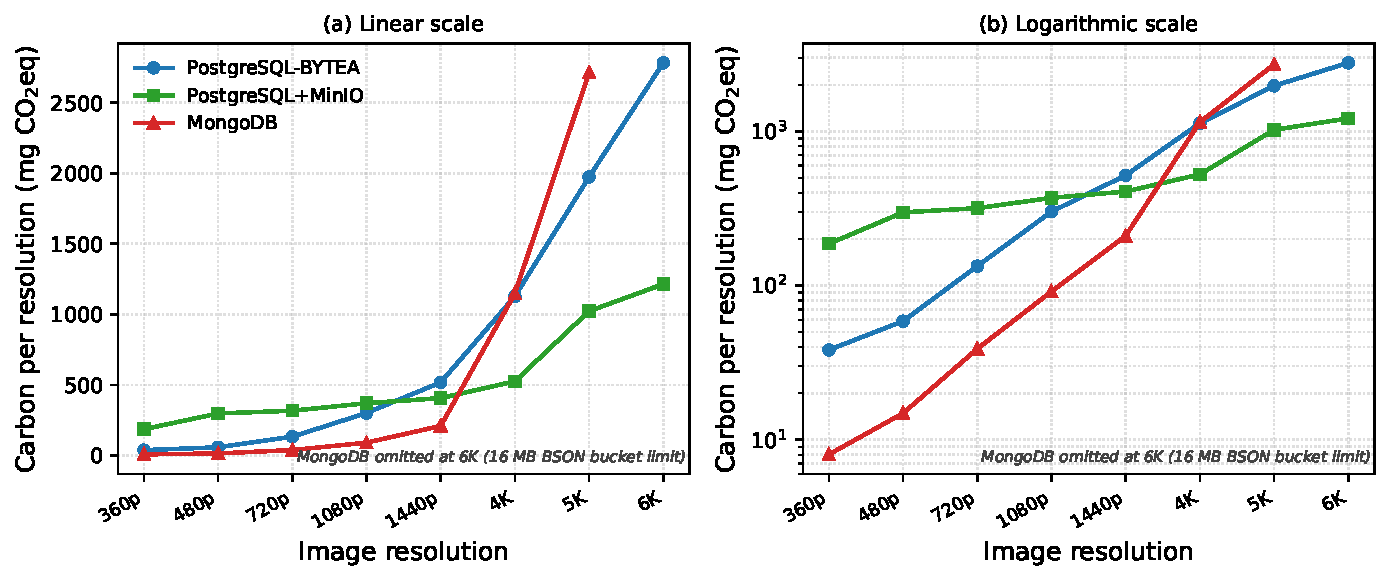
\includegraphics[width=\linewidth]{carbon_per_resolution.pdf}
\caption{Directly measured carbon per resolution (mg~CO\textsubscript{2}eq; insertion, bulk retrieval, and latest-frame read), on linear (left) and logarithmic (right) axes. MongoDB is greenest at $\le$1440p and the hybrid at $\ge$4K; MongoDB is omitted at 6K (Section~\ref{subsec:bson}).}\label{fig:carbon}
\end{figure}

\begin{table}[htbp]
\caption{Directly measured carbon per resolution for one run: 2{,}000 inserts, one 2{,}000-image bulk retrieval, and one latest-frame read (mg~CO\textsubscript{2}eq), each tracker's integrated measurement divided by its five runs. Bold marks the greenest.}\label{tab:carbon}
\small
\begin{tabular}{@{}lrrrl@{}}
\toprule
Res. & Postgre (BYTEA) & Mongo & PostMin (Postgre+MinIO) & Greenest \\
\midrule
360p  & 38.2    & \textbf{8.0}    & 186.6   & Mongo \\
480p  & 58.7    & \textbf{14.8}   & 298.2   & Mongo \\
720p  & 133.6   & \textbf{38.9}   & 317.6   & Mongo \\
1080p & 301.5   & \textbf{91.5}   & 370.5   & Mongo \\
1440p & 518.5   & \textbf{209.7}  & 407.0   & Mongo \\
4K    & 1128.0  & 1147.9 & \textbf{525.6} & PostMin \\
5K    & 1973.3  & 2712.9 & \textbf{1022.7} & PostMin \\
6K    & 2781.7  & --     & \textbf{1214.4} & PostMin \\
\midrule
\multicolumn{1}{@{}l}{Cum.\ 360p--5K} & 4151.8 & 4223.7 & \textbf{3128.2} & PostMin \\
\botrule
\end{tabular}
\footnotetext{Cumulative row over the common three-way range.}
\end{table}

\textbf{Carbon by operation.} The crossover recurs within each operation (Table~\ref{tab:dimcarbon}). The operational Software Carbon Intensity of ingestion~\citep{gsf_sci}, per 1{,}000 stored frames, spans nearly three orders of magnitude and inverts between engines: 2.7~mg for MongoDB against 83.6~mg for the hybrid at 360p, but 467~mg for the hybrid against 1{,}167~mg for MongoDB at 5K. For bulk retrieval MongoDB is greenest up to 720p and the hybrid from 1080p, earlier than for insertion, because HTTP streaming keeps large values out of the database engine. Latest-frame reads cost under 1~mg throughout (Online Resource~1).

\begin{table}[htbp]
\caption{Carbon by operation (mg~CO\textsubscript{2}eq): ingestion per 1{,}000 stored frames, the operational term of Software Carbon Intensity, and one 2{,}000-image bulk retrieval. Bold marks the greenest; embodied carbon is treated in Section~\ref{subsec:grid}.}\label{tab:dimcarbon}\label{tab:sci}
\small
\setlength{\tabcolsep}{4pt}
\begin{tabular}{@{}lrrrrrr@{}}
\toprule
 & \multicolumn{3}{c}{Ingestion, per 1{,}000 frames} & \multicolumn{3}{c}{Bulk retrieval, per run} \\
\cmidrule(lr){2-4}\cmidrule(lr){5-7}
Res. & Postgre & Mongo & PostMin & Postgre & Mongo & PostMin \\
\midrule
360p  & 13.6 & \textbf{2.7} & 83.6 & 11.0 & \textbf{2.6} & 19.4 \\
480p  & 20.0 & \textbf{4.4} & 139.1 & 18.8 & \textbf{6.0} & 19.8 \\
720p  & 47.0 & \textbf{12.3} & 147.4 & 39.5 & \textbf{14.2} & 22.8 \\
1080p & 103.4 & \textbf{28.8} & 170.6 & 94.5 & 33.8 & \textbf{29.2} \\
1440p & 184.0 & \textbf{75.4} & 184.0 & 150.4 & 58.9 & \textbf{38.9} \\
4K    & 399.3 & 506.2 & \textbf{232.0} & 329.2 & 135.2 & \textbf{61.6} \\
5K    & 686.1 & 1166.8 & \textbf{466.6} & 600.7 & 378.5 & \textbf{89.4} \\
6K    & 963.4 & -- & \textbf{542.6} & 854.4 & -- & \textbf{129.1} \\
\botrule
\end{tabular}
\end{table}

\textbf{Embodied carbon of storage amplification.} Provisioned storage also carries manufacturing carbon~\citep{gupta_chasing_carbon,tannu_ssd_embodied}. At 5K, 2{,}000 frames are $10.7$~GB of payload; the hybrid provisions essentially that, inline PostgreSQL $\approx$11.1~GB, and MongoDB, at $3.00\times$ amplification, $\approx$32.0~GB. At 0.16~kg~CO\textsubscript{2}eq per GB of flash~\citep{tannu_ssd_embodied}, MongoDB carries $\approx$5.1~kg of embodied carbon for these data against $\approx$1.7~kg for the hybrid. This first-order estimate covers the storage medium alone and scales linearly with capacity; Section~\ref{subsec:grid} shows that for retained frames it can outweigh the operational figures.

\subsection{Sensitivity of the ranking}\label{subsec:grid}
Online Resource~2 varies, one at a time, the factors on which the ranking could depend, using the measured cells of all six data sets; no benchmark was re-run. Table~\ref{tab:robustness} summarises the outcome. Grid intensity and PUE multiply every architecture's carbon by the same factor, so they cannot reorder the architectures: across seven national grids from 41 to 713~g/kWh~\citep{owid_carbon_intensity} the hybrid keeps the lowest cumulative 360p--5K footprint, and only the absolute saving changes. The operation mix leaves every collage result unchanged on both hosts and matters only at the deployment's own payload, where inline PostgreSQL wins ingestion-heavy workloads and MongoDB anything more read-heavy. Run-to-run variability overturns no winner on the larger host; on the smaller one it turns the nine cells nearest a crossover into ties, which blurs where a boundary falls without changing which architectures it separates. The largest effect comes from outside the operational boundary of Table~\ref{tab:boundary}: the embodied carbon of the retained frames. At 5~frames per second, even 30 days of retention carries 4 to 16 times the operational carbon of writing the frames on hard disks and 29 to 125 times on flash. It changes the choice only where the operational winner keeps more bytes on disk than a close rival, most notably at the deployment's own payload (Section~\ref{subsec:applied}).

\begin{table}[htbp]
\caption{Sensitivity of the architecture ranking: each factor varied alone over the measured cells of all six data sets (Online Resource~2).}\label{tab:robustness}
\small
\begin{tabular}{@{}L{0.2\textwidth}L{0.33\textwidth}L{0.4\textwidth}@{}}
\toprule
Factor & Range tested & Does the choice change? \\
\midrule
Operation mix & 0--10 bulk retrievals and 0--2{,}000 latest-frame reads per 2{,}000 inserts & Collage, either host: no. Real frames: only at the networked camera's 1080p payload \\
Run-to-run variability & Each operation perturbed by its own run-to-run spread & No winner overturned on the i9; nine cells at a crossover on the i7 become ties \\
Embodied carbon of retained frames & 0.02 (HDD) and 0.16 (SSD) kg~CO\textsubscript{2}eq/GB~\citep{tannu_ssd_embodied}, 30--365 days & Only where the operational winner keeps more bytes than a close rival \\
Grid intensity & 41--713~g/kWh, seven national grids & No \\
PUE & 1.0--2.0 & No \\
Frame rate and camera count & Any & No; savings scale linearly \\
Host and corpus & Two hosts; collage and three real cameras & Ordering holds; the crossover moves (Sections~\ref{subsec:twohosts} and~\ref{subsec:sizevsres}) \\
\botrule
\end{tabular}
\end{table}

\subsection{The MongoDB 16~MiB ceiling}\label{subsec:bson}
MongoDB could not store 6K frames at all. The 6K payload is 7.13~MB, well within the 16~MiB limit on one BSON document, yet insertion failed with error~10334 (\texttt{BSONObjectTooLarge}) on an object of 22.4~MB, about three payloads. Native Time-Series Collections \emph{bucket} measurements that share a metadata value into one bucket document, itself bound by the 16~MiB limit; with multi-megabyte payloads only two frames fit, and bucketing a third breaches the ceiling. Two things should be kept apart. The ceiling on a single document is fixed by the specification, and no configuration or hardware raises it. Whether several frames are combined into a document that exceeds it depends on configuration: we use the default bucketing with one metadata value shared by every row, which is what a practitioner obtains without deliberate tuning. Under it, MongoDB inline storage is \emph{infeasible} at 6K whatever the cache or machine; a different bucket span or a higher metadata cardinality might postpone the failure, which we did not test. A second limit, which does depend on the host, is reported in Section~\ref{subsec:memory}.

\subsection{The same payloads on two machines}\label{subsec:twohosts}
Repeating the collage sweep on a markedly smaller machine (an i7 with 8 threads and 15~GB, against the i9's 16 threads and 31~GB) tests whether the ordering belongs to the architectures or to the host. Payloads, database images, and protocol are identical, while hardware and software versions differ, so the comparison varies the environment rather than isolating the processor (Online Resource~1). Three results follow (Table~\ref{tab:twohosts}). The ordering at small payloads is unchanged: MongoDB has the lowest ingestion carbon up to $0.80$~MB on both machines. Its advantage runs out earlier on the smaller machine: at $1.40$~MB it emits $0.41\times$ the hybrid's ingestion carbon on the i9 but $1.01\times$ on the i7, a tie rather than a crossover, though a margin of more than a factor of two has gone, as the mechanism of Section~\ref{subsec:model} predicts. And MongoDB stops being runnable on the smaller machine from 4K (Section~\ref{subsec:memory}), while the other two complete every payload to $7.13$~MB.

\begin{table}[htbp]
\caption{The same collage payloads on both hosts: amortised ingestion carbon (mg~CO\textsubscript{2}eq per frame). Bold marks the lowest in each row, except where two are within measurement variability; processor, memory, storage, and software versions differ (Online Resource~1).}\label{tab:twohosts}
\small
\setlength{\tabcolsep}{4pt}
\begin{tabular}{@{}lr rrr rrr@{}}
\toprule
 & & \multicolumn{3}{c}{i9, 16 threads, 31~GB} & \multicolumn{3}{c}{i7, 8 threads, 15~GB} \\
\cmidrule(lr){3-5}\cmidrule(lr){6-8}
Resolution & MB & Postgre & PostMin & Mongo & Postgre & PostMin & Mongo \\
\midrule
360p  & 0.09 & 0.0136 & 0.0836 & \textbf{0.0027} & 0.0087 & 0.0277 & \textbf{0.0020} \\
480p  & 0.16 & 0.0200 & 0.1391 & \textbf{0.0044} & 0.0146 & 0.0431 & \textbf{0.0049} \\
720p  & 0.36 & 0.0470 & 0.1474 & \textbf{0.0123} & 0.0314 & 0.0608 & \textbf{0.0184} \\
1080p & 0.80 & 0.1034 & 0.1706 & \textbf{0.0288} & 0.0748 & 0.0928 & \textbf{0.0365} \\
\midrule
1440p & 1.40 & 0.1840 & 0.1840 & \textbf{0.0754} & 0.1889 & 0.1274 & 0.1287 \\
4K    & 2.99 & 0.3993 & \textbf{0.2320} & 0.5062 & 0.4401 & \textbf{0.2186} & failed \\
5K    & 5.09 & 0.6861 & \textbf{0.4666} & 1.1668 & 0.7730 & \textbf{0.4024} & --- \\
6K    & 7.13 & 0.9634 & \textbf{0.5426} & failed & 1.1198 & \textbf{0.4659} & --- \\
\botrule
\end{tabular}
\footnotetext{Above the rule the ordering is identical on both hosts; below it the hybrid takes over one payload step earlier on the smaller. ``failed'': attempted and terminated, by the BSON ceiling at 6K (Section~\ref{subsec:bson}) or by memory exhaustion at 4K on the smaller host (Section~\ref{subsec:memory}); ``---'': not attempted. The coefficient of variation of insertion time reaches 49\% on the smaller host (MongoDB, 720p) against under 8\% on the larger.}
\end{table}

\subsection{A second infeasibility: memory, not protocol}\label{subsec:memory}
The smaller host revealed a second limit, different in kind from the BSON ceiling of Section~\ref{subsec:bson} and met much sooner. There MongoDB completed 360p to 1440p, its ingest rate falling from $3{,}973$ to $28.9$~rows/s; at 4K it collapsed to three to five rows per second before the kernel's out-of-memory killer terminated \texttt{mongod}, twice, and the cell was recorded as skipped, while the other two completed 6K. WiredTiger keeps documents uncompressed in cache, so one 2{,}000-frame run at 4K is $5.8$~GB of live working set, whereas TOAST moves the payload out of line and the hybrid never admits it to the database. The cache had the same share of memory on both hosts and neither had swap, so a more conservative cache would probably have completed the sweep more slowly (Online Resource~1). On constrained hardware, whether an architecture runs at all comes before the margins between those that do.

\subsection{Reinforcing the results with a real-case deployment}\label{subsec:realframes}
The benchmark above inserts one deterministic collage per resolution in every row, so all 2{,}000 stored rows are byte-identical. That makes it exactly reproducible but unlike camera output, since identical rows are compressible in a way real data are not. We therefore repeat it on real frames recorded from a \emph{face-recognition-based attendance system} in operational use, with one networked camera and two USB cameras, inserting a different frame in every row. Its recognition pipeline lies outside this paper, so the figures are those of the data tier alone. Ten minutes of capture at 5~frames per second yielded 2{,}845--2{,}988 byte-distinct frames per camera, in which an automated sweep detected no faces (see the ethics statement). The benchmark ran on the smaller host of Section~\ref{subsec:twohosts}, and Online Resource~1 describes the cameras and the application that recorded them.

Three findings follow (Table~\ref{tab:realframes} and Figure~\ref{fig:realframes}). First, \textbf{the architectural conclusion holds under the equal-weight profile}: MongoDB is the lowest-carbon architecture at every resolution from 360p to 1080p, as in the collage sweep, and the result replicates on a second camera. Second, \textbf{real payloads are far smaller than the collage}, by $3.1\times$ at 360p rising to $5.4\times$ at 1080p, so the quality-90 collage is close to a worst case for compressibility. Third, \textbf{storing one repeated image rather than distinct ones overstates MongoDB's advantage}. At approximately matched payload size on the same host (Online Resource~1), MongoDB's ingestion carbon rises by $2.4$ to $2.9\times$ with distinct frames, while PostgreSQL and the hybrid become cheaper; its measured storage amplification rises far more, although those readings are uncertain (Section~\ref{subsec:threats}). The asymmetry is consistent with cross-row compression: MongoDB alone groups many frames into one bucket document, where repeated content can be compressed together, whereas TOAST compresses per value and MinIO stores per object.

\begin{figure}[htbp]
\centering
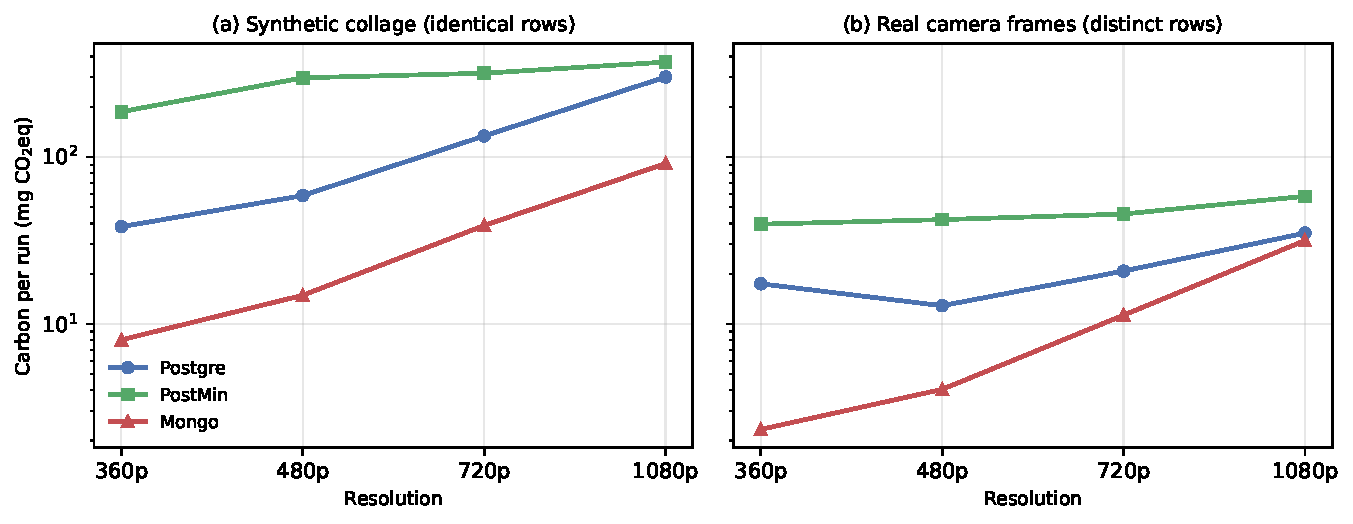
\includegraphics[width=\linewidth]{realframes_carbon.pdf}
\caption{Carbon per run against resolution for the single-image collage (a) and real camera frames (b), on a logarithmic axis. The ordering is the same in both panels, with MongoDB lowest throughout under the equal-weight profile; with distinct real frames its margin over inline PostgreSQL narrows as resolution rises, to 11\% at 1080p.}\label{fig:realframes}
\end{figure}

\begin{table}[htbp]
\caption{Real recorded camera frames versus the single-image collage, 360p--1080p, on the networked camera. Carbon is the per-run total of insertion, bulk retrieval, and latest-frame read. ``Amp'' is MongoDB's storage amplification, a single reading per cell (Section~\ref{subsec:threats}). Every real-frame row holds a different photograph.}\label{tab:realframes}
\small
\begin{tabular}{@{}lrrrrrr@{}}
\toprule
 & \multicolumn{2}{c}{Payload (MB)} & \multicolumn{2}{c}{Mongo carbon (mg)} & \multicolumn{2}{c}{Mongo amp ($\times$)} \\
\cmidrule(lr){2-3}\cmidrule(lr){4-5}\cmidrule(lr){6-7}
Resolution & Collage & Real & Collage & Real & Collage & Real \\
\midrule
360p  & 0.09 & 0.03 &  8.03 &  2.33 & 0.001 & 0.000 \\
480p  & 0.16 & 0.05 & 14.84 &  4.05 & 0.000 & 0.000 \\
720p  & 0.36 & 0.09 & 38.85 & 11.28 & 0.101 & \textbf{0.274} \\
1080p & 0.80 & 0.15 & 91.46 & 31.59 & 0.101 & \textbf{0.924} \\
\botrule
\end{tabular}
\footnotetext{Under the equal-weight profile MongoDB has the lowest total in every row of both runs, and on the second camera as well: at 1080p the three real-frame totals are $31.59$ (Mongo), $34.99$ (Postgre), and $58.17$~mg on this camera, and $18.82$, $29.94$, and $90.42$~mg on the external USB camera. Storage amplification for PostgreSQL ($1.03$--$1.09\times$) and the hybrid ($1.00$--$1.02\times$) is unchanged by payload realism.}
\end{table}

The two corpora therefore agree on \emph{which} architecture to choose over most of the range and differ on \emph{by how much}: with real payloads MongoDB's margin narrows as resolution rises, so the crossover to the hybrid should come earlier than on the collage. Real frames differ from the collage in size as well as in distinctness, so the matched-size comparison is the cleanest attribution available rather than a controlled isolation.

\subsection{Payload size, not resolution, determines the outcome}\label{subsec:sizevsres}
The results so far are indexed by resolution, which is how cameras are specified, but the two corpora show that resolution is only a label for the deciding variable, the payload. Three observations establish this.

\textbf{The same resolution produces very different payloads.} A 1080p frame is $0.804$~MB as a quality-90 collage and $0.149$~MB as ordinary camera output, and across 360p to 1080p the factor runs from $3.1$ to $5.4$.

\textbf{Even two real cameras disagree.} The networked camera and the USB camera differ by $12.3\%$ in encoded size at 1080p, and the sign reverses at 720p: the networked camera's H.264 stream carries more high-frequency content, which survives at native resolution and is removed by downscaling.

\textbf{The consequence is a different architecture.} At 1080p on one host, under an ingestion-only profile, the collage payload selects MongoDB and the networked camera's output selects inline PostgreSQL. The USB camera's 1080p output, $0.131$~MB, still selects MongoDB, whereas the networked camera's $0.149$~MB does not, so together they place the transition between those payloads, both labelled 1080p.

We therefore state the decision rule in Section~\ref{sec:framework} in measured payload size and treat resolution as an indicative guide specific to the camera and the scene, since a rule calibrated in resolutions mis-selects for any camera whose payloads differ from its calibration.

%%=====================================================================%%
\section{A Carbon-Aware Decision Framework}\label{sec:framework}
%%=====================================================================%%

\subsection{Which architecture wins each operation}\label{subsec:winners}
Two regularities across the operations motivate a single decision rule. First, for insertion and bulk retrieval, which dominate the footprint, the lowest-carbon architecture is also the fastest at every payload measured, because those operations are long enough that elapsed time dominates and energy is power integrated over time; part of that correspondence is built into the measurement, since memory power is a constant estimate (Section~\ref{subsec:carbon_method}). It fails for latest-frame reads: at 360p and 720p the hybrid returns the frame fastest while MongoDB emits least, and at 480p inline PostgreSQL is fastest while MongoDB is again the greenest (Online Resource~1), because in a read of one to two milliseconds differences in average power outweigh differences in time.

Second, every operation shows the same MongoDB--hybrid scissors, differing only in where the blades cross: storage and insertion at the largest payloads, bulk retrieval earlier, while latest-frame reads favour the hybrid across almost the whole range. On the collage payloads inline PostgreSQL is the greenest at no single operation, and in bulk retrieval it is both the slowest and the highest-carbon architecture from 720p up (Tables~\ref{tab:read} and~\ref{tab:dimcarbon}). Like the hybrid, it completes the full payload range on both machines, which MongoDB does not (Sections~\ref{subsec:bson} and~\ref{subsec:memory}). We do not tabulate these crossovers by resolution, because where they fall is a property of the camera and the corpus (Section~\ref{subsec:sizevsres}).

\subsection{Selecting an architecture by operating regime}\label{subsec:selection}
The decision variable is the payload a camera actually produces (Section~\ref{subsec:sizevsres}); the secondary variable is workload emphasis: write-heavy ingestion, read-heavy analytics, or storage-bound archival. Table~\ref{tab:decision} states the rule, with the resolutions that produce each payload under the high-entropy collage shown as an indicative guide only; the boundaries for a particular installation are located by the procedure of Section~\ref{subsec:model}.

\begin{table}[htbp]
\caption{Carbon-aware architecture selection. The regime is set by measured payload size; the resolutions in parentheses produce that payload under the high-entropy collage and are indicative only, since a real camera at the same resolution usually produces a lighter payload. Postgre = PostgreSQL-BYTEA; Mongo = MongoDB; PostMin = PostgreSQL+MinIO.}\label{tab:decision}
\small
\begin{tabular}{@{}p{0.30\textwidth}p{0.12\textwidth}p{0.44\textwidth}@{}}
\toprule
Operating regime (payload per frame) & Choice$^{\ast}$ & Rationale \\
\midrule
Below the measured ingestion crossover, ingest-heavy & Mongo & Greenest where its near-zero per-operation overhead dominates: bucketed writes with no per-object network call. The boundary is $1.4$--$3.0$~MB for worst-case payloads but $0.09$--$0.15$~MB for real camera output, so \emph{measure before assuming this row applies}. \\
Above that boundary but below $\approx$3~MB ($\approx$4K), ingest-heavy & Postgre & MongoDB's per-byte cost ($\approx$2.5$\times$ the hybrid's) has overtaken its overhead advantage, while the hybrid's per-object HTTP cost is not yet amortised. \\
$\gtrsim$3~MB ($\gtrsim$4K), any emphasis & PostMin & $\sim$half the carbon of inline storage; flat storage amplification; HTTP streaming makes reads cheap once the payload is large. \\
Mixed or unmeasured payloads & Postgre & Stays within $4.8\times$ of the greenest choice at every payload, while the hybrid, the only other architecture that completes every payload on both hosts, reaches $23\times$ (Table~\ref{tab:carbon}; $3.6$--$4.4\times$ against $12$--$39\times$ on the other data sets). Single transactional boundary; the safe default when payloads are unmeasured. \\
Storage-bound / archival (frames kept for weeks) & PostMin; Mongo below the crossover & The embodied carbon of the retained volume then outweighs write energy (Online Resource~2), so on-disk size decides. The hybrid stores $1.00$--$1.02\times$ the payload at every size and inline PostgreSQL $1.03$--$1.09\times$; MongoDB reaches $3.00\times$ at 5K, but below the crossover its measured footprint is at most $1.03\times$ and it also writes for less. \\
Large payloads, read-heavy & PostMin & Object streaming keeps latest-frame and bulk-retrieval latency and energy low. \\
$\gtrsim$3~MB per frame on a memory-constrained host & Postgre or PostMin & MongoDB may be \emph{unrunnable} rather than merely costly: its uncompressed working set scales with the payload, and on a 15~GB host it was terminated by the kernel at 4K while the other two completed 6K (Section~\ref{subsec:memory}). \\
$\gtrsim$7~MB per frame ($\gtrsim$6K)$^\dagger$ & Postgre or PostMin & MongoDB \emph{infeasible} under the tested time-series configuration: bucketed documents exceed the 16~MiB BSON limit, which no hardware raises. \\
\botrule
\end{tabular}
\footnotetext{$^{\ast}$Choices assume the equal-weight profile of Table~\ref{tab:carbon} unless the regime names an emphasis; where a deployment writes far more often than it reads, the choice may differ (Section~\ref{subsec:applied}). $^\dagger$One 6K frame is within the 16~MiB limit; the limit is breached because bucketing groups several multi-megabyte frames into one bucket document (Section~\ref{subsec:bson}), on any hardware.}
\end{table}

\subsection{Why the crossover exists, and how to locate it elsewhere}\label{subsec:model}
The rule is stated in payload sizes measured on our hardware, but the mechanism behind it is not hardware-specific, which is what allows the rule to be relocated rather than copied. Each architecture pays a \emph{fixed} cost per operation regardless of payload (a network round-trip, a transaction boundary, an index update) and a \emph{payload-dependent} cost that grows with the bytes moved and written. MongoDB has the smallest fixed cost, since inserts are batched into shared buckets with no per-object network call, but the steepest payload growth: WiredTiger writes the whole document, image included, through its B-tree pages and holds it uncompressed in cache~\citep{wiredtiger_btree_architecture}. The hybrid is the mirror image, paying one HTTP \texttt{PUT} per frame but then streaming the object while PostgreSQL writes only metadata. Inline PostgreSQL lies between the two on both counts, so it wins at neither end of the range. Its bulk retrieval, however, is the most expensive from 720p up, and at 1440p, where its insertion matches the hybrid's (Table~\ref{tab:twohosts}), that gives it the highest total of the three (Table~\ref{tab:carbon}).

The lowest fixed cost therefore wins at small payloads and the shallowest growth at large ones, so the curves cross. This is a statement about ordering, not functional form. MongoDB's per-frame cost rises by more than two orders of magnitude across the measured range and accelerates sharply above about one megabyte, as the cache fills and eviction begins to stall writes~\citep{percona_wiredtiger_eviction} (Figure~\ref{fig:crossover_collage}); a straight line fitted across that range produces negative intercepts, so we report no closed-form law, only the ordering of the regimes and the interval in which each transition occurs. Where a transition falls depends on both payload and host: changing the payload construction on one host introduces a transition at a payload an order of magnitude smaller (Section~\ref{subsec:sizevsres}), and changing the host moves it by one resolution step (Section~\ref{subsec:twohosts}). The boundary is therefore something an adopter locates rather than inherits.

The sequence of regimes is stable, with the intermediate architecture winning a band between the two ends when payloads are realistic enough for it to open, but the boundaries are not constants. Locating them needs measurement at a few payload sizes, the bracketing procedure used here, and no model:

\begin{enumerate}\setlength{\itemsep}{1pt}\setlength{\parskip}{0pt}
  \item \emph{Measure the payload.} Record a few minutes from the cameras to be deployed and take the mean and spread of the encoded frame size. This, not the advertised resolution, is the decision variable (Section~\ref{subsec:sizevsres}).
  \item \emph{Fix the operation profile and the retention.} State how many insertions, bulk retrievals, and point reads a representative period of operation contains, and how long frames are kept. A continuously capturing installation is close to ingestion-only and an analytics tier is not, and the choice changes the answer (Section~\ref{subsec:applied}); beyond a few days of retention, the embodied carbon of the stored volume can decide it (Section~\ref{subsec:grid}).
  \item \emph{Bracket.} Measure each candidate at three or four payload sizes spanning that range, with at least one below and one above it, under the chosen profile.
  \item \emph{Compare with uncertainty.} Repeat enough runs to estimate run-to-run variability, and treat any separation inside it as a tie rather than a winner, as Online Resource~2 does cell by cell; on our smaller host the coefficient of variation reached $58\%$.
  \item \emph{Exclude infeasible cells.} An architecture that fails to complete a payload is excluded at that payload and above, not scored on the runs that did complete.
  \item \emph{Select} the lowest architecture across the bracketed range, and repeat if the payload estimate or the operation profile changes materially.
\end{enumerate}

\noindent What transfers between installations is this procedure and the sequence of regimes it recovers, not the payload sizes at which our own boundaries happen to fall. Two claims are stronger than any measured boundary, because they do not depend on measurement: the 16~MiB BSON ceiling is a protocol limit (Section~\ref{subsec:bson}), and the ordering of payload-dependent costs follows from where each architecture places the payload rather than from how fast the host runs.

\subsection{Applying the framework to the deployment}\label{subsec:applied}
We close by applying the framework to the deployment that supplied the corpus of Section~\ref{subsec:realframes}, using its measured payload of $0.149$~MB at 1080p. The camera captures continuously at 5~frames per second, $1.577\times10^{8}$ stored frames a year, and the annual figures are a \emph{scenario projection} obtained by scaling measured per-frame rates, not a saving measured against the installation as it runs. Figures are per camera (Figure~\ref{fig:applied} and Table~\ref{tab:applied}; Online Resource~1 plots the annual totals).

\begin{figure}[htbp]
\centering
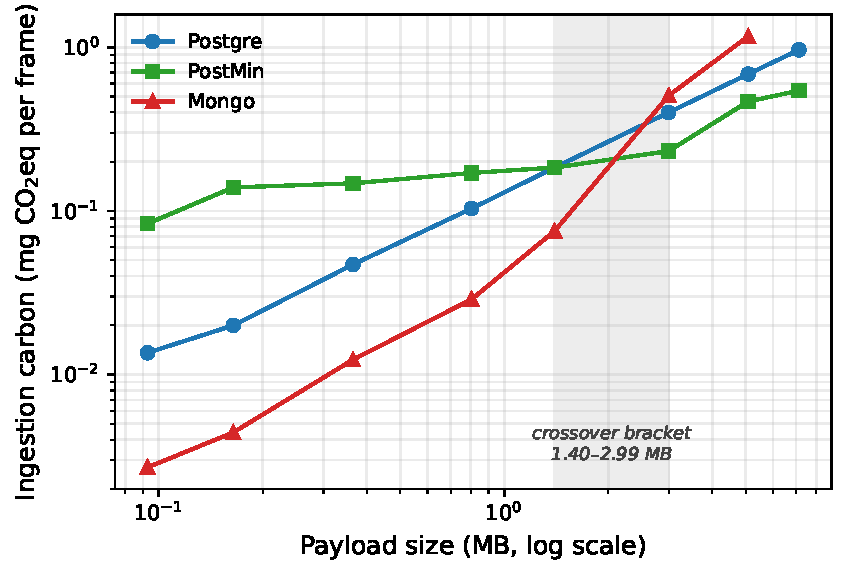
\includegraphics[width=\linewidth]{crossover_collage.pdf}
\caption{Ingestion carbon against payload size across the collage range, on logarithmic axes; lines join measurements and imply no functional form. MongoDB's per-frame cost rises by more than two orders of magnitude and accelerates beyond about one megabyte. Shading marks the bracket in which the lowest-carbon architecture changes from MongoDB to the hybrid; MongoDB is absent at 6K, where it is infeasible (Section~\ref{subsec:bson}).}\label{fig:crossover_collage}
\end{figure}

\begin{figure}[htbp]
\centering
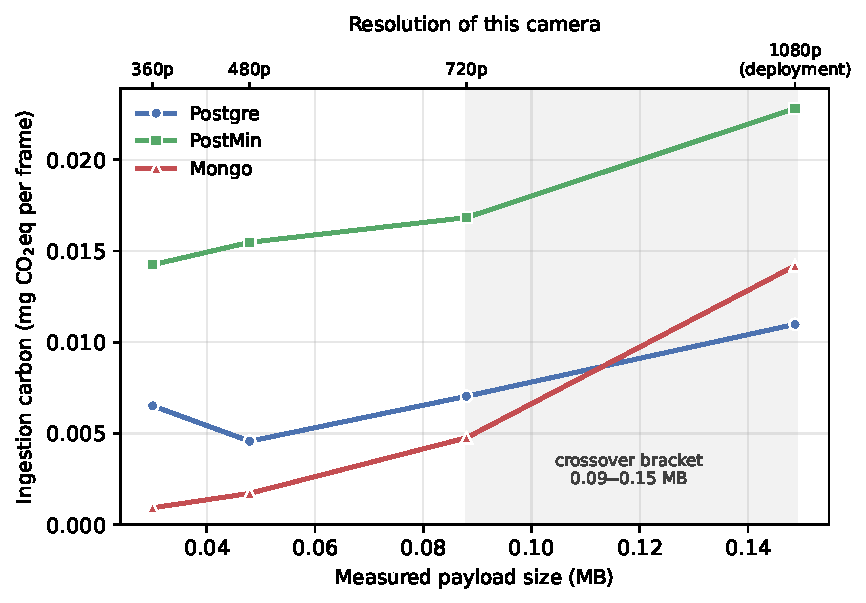
\includegraphics[width=\linewidth]{crossover_realcase.pdf}
\caption{The same measurement for the real-frame corpus, over the payloads the deployment produces; the upper axis shows where this camera's resolutions fall, a relation specific to the camera. The crossover bracket lies between $0.09$ and $0.15$~MB, an order of magnitude below the collage bracket of Figure~\ref{fig:crossover_collage}, and the deployment operates at its upper edge.}\label{fig:applied}
\end{figure}

\begin{table}[htbp]
\caption{The framework applied to one camera of the deployment as a scenario projection: 1080p, 5~frames per second, continuous capture, measured payload $0.149$~MB. Carbon is per camera per year; ``write'' counts ingestion only and ``total'' adds bulk retrieval and latest-frame reads; storage is the volume retained at 90 days.}\label{tab:applied}
\small
\begin{tabular}{@{}lrrrr@{}}
\toprule
Architecture & mg/frame & kg/yr (write) & kg/yr (total) & TB at 90 days \\
\midrule
Postgre & \textbf{0.0110} & \textbf{1.73} & 2.76 & 5.96 \\
Mongo   & 0.0142 & 2.24 & \textbf{2.49} & \textbf{5.34} \\
PostMin & 0.0228 & 3.60 & 4.59 & 5.79 \\
\botrule
\end{tabular}
\end{table}

Three observations follow.

\textbf{The answer depends on the measured payload.} For this deployment the framework selects inline PostgreSQL, not MongoDB, although 1080p would sit in MongoDB's band if the bands were read as resolutions calibrated on the collage. This camera's payload sits at the upper edge of the crossover bracket measured on real frames, between $0.131$ and $0.149$~MB (Section~\ref{subsec:sizevsres}), on PostgreSQL's side, and the annual figures confirm it, at $1.73$ against $2.24$~kg per camera. A resolution-only rule would have missed the boundary entirely.

\textbf{Workload emphasis changes the answer.} Ingestion alone selects PostgreSQL; counting retrieval and latest-frame reads equally selects MongoDB ($2.49$ against $2.76$~kg), and so does minimising retained volume ($5.34$~TB at 90 days). A deployment that stores continuously and reads rarely, as this one does, is governed by the write column.

\textbf{Retention can override both.} The projection counts operation alone. At 90 days of retention one camera keeps about 6~TB, whose embodied carbon, spread over a five-year drive life, comes to about 23~kg a year on hard disks and 185 to 191~kg on flash, far above the operational figures. Counted in, it favours the smallest footprint, here MongoDB's, once retention exceeds 2 to 8 days on flash (Online Resource~2). The selection above therefore holds for the operational carbon of ingestion, and a site that keeps frames for weeks should weigh footprint first.

Two boundaries apply. The installation currently retains video rather than individual frames, so these figures project an image-based tier for it rather than a saving against its present configuration. And the projection scales the measured energy per stored frame, which includes the host's background draw only while the benchmark worked on each frame; a host running all year also draws power between frames, which the projection leaves out.

%%=====================================================================%%
\section{Discussion}\label{sec:discussion}
%%=====================================================================%%

\subsection{Implications and operational trade-offs}
There is no single ``green database'': the answer depends on the operation profile and the retention as much as on the payload. Under the equal-weight profile, light camera streams are greenest on MongoDB and heavy inspection or surveillance streams on PostgreSQL+MinIO. For a continuously capturing installation, real camera payloads put inline PostgreSQL ahead at ingestion near 0.15~MB (Section~\ref{subsec:applied}), and keeping frames for weeks hands the choice to on-disk footprint (Section~\ref{subsec:grid}). Inline PostgreSQL is the safe default when payloads are unmeasured, and MongoDB is out of consideration from 6K under default bucketing, whatever its carbon.

Operational costs weigh against the hybrid's advantages at high resolution. It runs two services with independent failure modes, and its write is not atomic: a crash between the database insert and the MinIO upload can leave an image without its metadata or the reverse, so orphaned objects need cleaning up. Inline PostgreSQL keeps everything in one all-or-nothing transaction. Because the mechanism, inline large-object handling against externalised object transport, is generic, the crossover should carry over to other relational engines with large-object columns, though the exact points depend on each engine's page layout and logging. Once the payload is externalised the metadata engine adds only a small, payload-independent overhead, so a MongoDB+MinIO hybrid would closely track PostgreSQL+MinIO, which is why the comparison keeps to the inline-versus-externalised axis.

\subsection{From measured savings to accounting, markets, and policy}\label{subsec:accounting}
\textbf{What the figures are.} They are measured operational emissions of one subsystem's electricity, converted with a national average grid factor, plus a first-order estimate of the storage medium's manufacturing carbon. In the terms of ISO~14067~\citep{iso_14067_cfp} they are closest to a \emph{partial} carbon footprint: emissions of selected processes from two life-cycle stages, use-stage electricity and medium production, reported per declared unit of 1{,}000 stored frames, rather than the footprint of a whole product system. They are not an organisational inventory under ISO~14064-1~\citep{iso_14064_1_inventory}, and they have not been verified as a greenhouse-gas statement under ISO~14064-3~\citep{iso_14064_3_verification}. SCI~\citep{gsf_sci,iso_iec_21031_sci} is a rate per functional unit that only eliminating emissions can lower; offsets and market instruments such as renewable energy certificates cannot.

\textbf{Component and service.} A lower storage-tier footprint lowers a service's footprint only if nothing else changes; Table~\ref{tab:boundary} lists what our figures leave out, and the hybrid in particular adds a second service whose idle draw and replication lie outside that boundary. Under the GHG Protocol, an operator that runs its own servers, including in colocation under its operational control, sees the saving in Scope~2~\citep{ghgp_scope2_guidance}: in full under location-based accounting, which uses average grid factors, and under market-based accounting only to the extent that its purchased electricity carries emissions. Its metered electricity also includes parts our measurement does not see, such as the storage device, power supply, and cooling. A cloud customer reports the provider's electricity in Scope~3, Category~1~\citep{ghgp_scope3_standard}, and sees the saving only if it uses supplier-specific data rather than spend-based estimates.

\textbf{Procurement and investment.} Carbon per 1{,}000 frames at the buyer's own measured payload can serve as a tender and supplier criterion, since it is measurable with the procedure of Section~\ref{subsec:model}. Storage amplification belongs in the same specification, because it sets the capacity to be bought and, with it, the embodied carbon that dominates for retained frames (Section~\ref{subsec:grid}). The choice is made once, at design time, and costs nothing to run.

\textbf{Inventories and national outcomes.} Our figures are estimated operational reductions for one subsystem. They enter an organisational inventory only through the Scope~2 or Scope~3 accounting above, and they reach national outcomes only as lower electricity demand, which already appears as lower power-sector emissions in the country's own inventory. They support a nationally determined contribution~\citep{unfccc_paris_agreement} only in that indirect sense. As grids decarbonise under national pledges, the operational saving shrinks with the grid factor, while the embodied part, set by provisioned capacity, does not.

\textbf{Savings are not carbon credits.} A credit under a programme such as the Verified Carbon Standard~\citep{verra_vcs_standard} needs an approved methodology, a justified baseline scenario, a demonstration of additionality, monitoring, and validation and verification by an accredited body, and it represents one verified tonne of CO\textsubscript{2}eq. A measured efficiency difference between two storage designs meets none of these by itself. Transferring such a reduction between countries would also require authorisation and a corresponding adjustment under Article~6 of the Paris Agreement, so that it is not counted twice~\citep{unfccc_paris_agreement,unfccc_decision_2cma3}. For scale, the deployment's saving is 0.28~t~CO\textsubscript{2}eq a year for a 100-camera site at a PUE of 1.5, under a third of one credit.

\textbf{Materiality.} Percentages alone overstate what is at stake per camera. At the deployment payload, inline PostgreSQL saves 0.51~kg a year per camera against the runner-up and 1.86~kg against the costliest option, $23\%$ and $52\%$ of the ingestion footprint; at a 4K payload the hybrid saves 26 to 43~kg per camera a year (Online Resource~2). The choice becomes material for large fleets, high resolutions, carbon-intensive grids, and long retention, where the embodied carbon of the stored frames dominates. It serves chiefly SDG~13 (climate action) and SDG~12 (responsible consumption and production) of the United Nations Sustainable Development Goals~\citep{un_sdg}.

\subsection{Positioning against prior work}
The contribution relative to the studies in Table~\ref{tab:relwork} is a reversal of one of their conclusions rather than a further benchmark. TSBS~\citep{tsbs} and the CrateDB benchmark~\citep{cratedb_ts_benchmark} rank systems on small scalar rows, and \citet{diva_timescaledb_mongodb_eval} report MongoDB ingesting faster than TimescaleDB on numeric sensor data. Our measurements agree at small payloads, where MongoDB ingests over $6\times$ faster than inline PostgreSQL at 360p, but the ordering inverts between 1440p and 4K, and MongoDB becomes infeasible at 6K. The comparison is qualitative, since those studies differ in data, hardware, and metrics; what it shows is that an ordering read in the scalar literature as a property of the engines belongs to the payload regime those benchmarks occupy. A practitioner choosing a store for images on the strength of scalar benchmarks would pick the architecture that is worst at scale, with no warning from the published evidence.

The carbon-accounting methods reviewed in Section~\ref{sec:related_work} attribute a footprint to a workload once its energy is known, but cannot say which architecture will consume least. Measuring per architecture, per operation, and per resolution is what exposes the crossover; one aggregate figure per architecture would have averaged it away and produced a spurious universal winner.

We therefore claim an inversion of the reported ordering in a payload regime the reviewed benchmarks do not reach, an infeasibility result that no hardware removes under default bucketing, and a transferable calibration procedure. We do not claim that the specific crossover payloads generalise: they are measurements on two hosts and a limited corpus, and Section~\ref{subsec:realframes} shows that even the margins depend on how realistic the payloads are.

\subsection{Threats to validity}\label{subsec:threats}
Three limits concern the measurements. First, each cell's carbon is one integrated CodeCarbon measurement normalised to one run, so it has no interval of its own; it is bounded instead by the run-to-run spread of the timed insertions and bulk retrievals, which stays under $8\%$ on the larger host but reaches $58\%$ on the smaller. The sensitivity analysis perturbs every cell by that spread (Section~\ref{subsec:grid}): no winner on the larger host changes, while nine cells near a crossover on the smaller host become ties, so the smaller host's crossovers are reported as margins rather than positions. Independent repeated energy runs would give each cell an interval. Second, only processor power is read from RAPL; memory power is CodeCarbon's estimate from installed capacity and makes up about a third to nearly three quarters of each cell's energy, so the energy figures are partly modelled, and the memory term rises with elapsed time. Third, MongoDB's storage amplification is a single \texttt{collStats} reading taken straight after insertion, without forcing a checkpoint. On distinct real frames it reads as low as $0.000$ at 360p and 480p, which cannot be the space 2{,}000 distinct JPEG frames occupy once written, so the small-payload readings understate MongoDB's footprint. The direction of the repetition effect (Section~\ref{subsec:realframes}) stands, but its size is uncertain, and the embodied-carbon analysis is repeated with amplification floored at $1.0$.

The scope is bounded by Table~\ref{tab:boundary}: the data tier of one host and container topology, one client issuing requests sequentially, and a batch size of 50. Since the crossover is driven by payload size, we expect neither concurrency nor larger batches to move the ordering, but neither was tested. The smaller host's MongoDB results stop at 1440p (Section~\ref{subsec:memory}), so its crossover is bracketed on one side only. The controlled payloads are collages built from one photograph~\citep{pexels_durdle_door}, paired with a real corpus from three cameras; a broader range of scenes would refine the absolute figures, though quality-90 photographs are already close to a worst case for the inline engines. Finally, the embodied-carbon and annual figures are first-order estimates from published factors and stated assumptions, and convey magnitude rather than site-specific values.

%%=====================================================================%%
\section{Conclusion}\label{sec:conclusion}
%%=====================================================================%%

This paper measured the carbon of storing image-based time-series data in MongoDB, inline PostgreSQL, and a PostgreSQL+MinIO hybrid from 360p to 6K, with a separate energy tracker for every architecture, operation, and resolution.

\emph{RQ1.} Under a profile weighting one insertion, one bulk retrieval, and one latest-frame read equally, MongoDB is greenest at standard resolutions and the hybrid from 4K, roughly halving the carbon of inline storage; inline PostgreSQL is never the greenest but stays within $4.8\times$ of it. MongoDB cannot store 6K frames under default bucketing, and on a memory-constrained host it fails from 4K. \emph{RQ2.} The ordering at small payloads holds on a second host and on real frames from three cameras; grid intensity and PUE cannot change it, while the operation mix and run-to-run variability matter only near a crossover. Counting the embodied carbon of retained frames changes the choice wherever the operational winner keeps more bytes than a close rival. \emph{RQ3.} The choice should be keyed to measured payload, operation profile, and retention, using the calibration procedure of Section~\ref{subsec:model}. The savings are reductions in a partial, unverified carbon footprint, which an operator running its own servers sees in Scope~2, and they are not carbon credits.

Four practical implications follow from Table~\ref{tab:decision}. Measure the payload before choosing, because a camera's output, not its resolution, sets the regime. A site that captures continuously and reads rarely should compare ingestion carbon, which near 0.15~MB favours inline PostgreSQL; if it keeps frames for more than a few days, it should choose by on-disk footprint instead, which favours MongoDB below the crossover and the hybrid above it. A memory-constrained host should avoid MongoDB for multi-megabyte frames, where it may not run at all. And a buyer should ask a vendor for carbon per 1{,}000 frames at the buyer's own payload, together with the storage amplification that sets capacity and embodied carbon.

Future work will extend the study to distributed and multi-client deployments, repeat the energy runs and measure idle draw so that every cell has an interval, re-measure MongoDB's storage at small payloads after a forced checkpoint, and broaden the real corpus above 1080p and across more scenes.

\backmatter

\section*{Statements and Declarations}

\textbf{Competing interests.} The authors declare no competing interests.

\textbf{Use of AI-assisted technologies.} Generative AI assistants (Google Gemini, Anthropic Claude via Claude Code, and OpenAI Codex) were used in an assistive capacity: supporting parts of the benchmark and analysis code, and improving the grammar, clarity, and phrasing of text written by the authors. Every measurement reported here is produced by the benchmark harness from hardware energy counters, and every table and figure is derived from those measurements by the scripts released with the artifact. No AI tool was used to interpret the experimental results or to draw the scientific conclusions reported here. The authors reviewed, verified, and edited all AI-assisted output and take full responsibility for the entire content of this manuscript. AI is not credited as an author, in accordance with the journal's editorial policy.

\textbf{Data and code availability.} A reproducibility artifact accompanies this submission and will be deposited in a public repository with a persistent identifier on acceptance. It contains the benchmark harness, the Docker configurations, the raw per-run measurement CSVs for all six measurement sets reported here (both hosts and all three cameras), the figure-generation scripts, and the manuscript source, so that every table and figure can be rebuilt without re-running the benchmark. The collage source image is redistributable under its original licence. The corpus of real camera frames used in Section~\ref{subsec:realframes} is released in full, as three archives of $2{,}845$, $2{,}988$, and $2{,}891$ frames, one per camera, alongside the recording tool that produced them; the frames are separated from the main archive only so that the code and measurements can be retrieved without them. Each measurement file records the country in which it was taken, since the grid-intensity factor depends on it, but not a finer location.

\textbf{Ethics.} The deployment described in Section~\ref{subsec:realframes} performs face recognition in normal operation, so we state precisely what was done. No recognition function was invoked and no enrolled identity, template, or record was accessed; the cameras were read directly, and the study used only the resulting image files as binary payloads. Recording was carried out by an author in a space with no other person present, and no biometric template was computed or stored at any point. Every saved frame was then passed through a face detector (YuNet, confidence threshold $0.35$) and none produced a detection. We report that as what it is: evidence that the released corpus contains \emph{no detectable faces}, not a proof that it contains no personal data, since a detector sweep cannot establish the latter. The frames are retained only as the study artifact and were not used for identification, recognition, tracking, or any purpose connected with the deployment's normal operation. Institutional guidance was that work of this kind, involving no participants and no processing of biometric data, does not require ethics review; we state the basis rather than assert an approval that was not sought. The images serve only as representative binary payloads for storage measurement, and no identification, recognition, or tracking was performed on them.

\bibliography{references}

\end{document}
